\documentclass[tikz,border=12pt]{standalone}
\usepackage[T1]{fontenc}
\usepackage{lmodern,amsmath,amssymb}
\usetikzlibrary{arrows.meta,positioning}
\definecolor{ink}{HTML}{183444}
\definecolor{blue}{HTML}{1B6780}
\definecolor{amber}{HTML}{AD601A}
\begin{document}
\hyphenpenalty=10000\exhyphenpenalty=10000
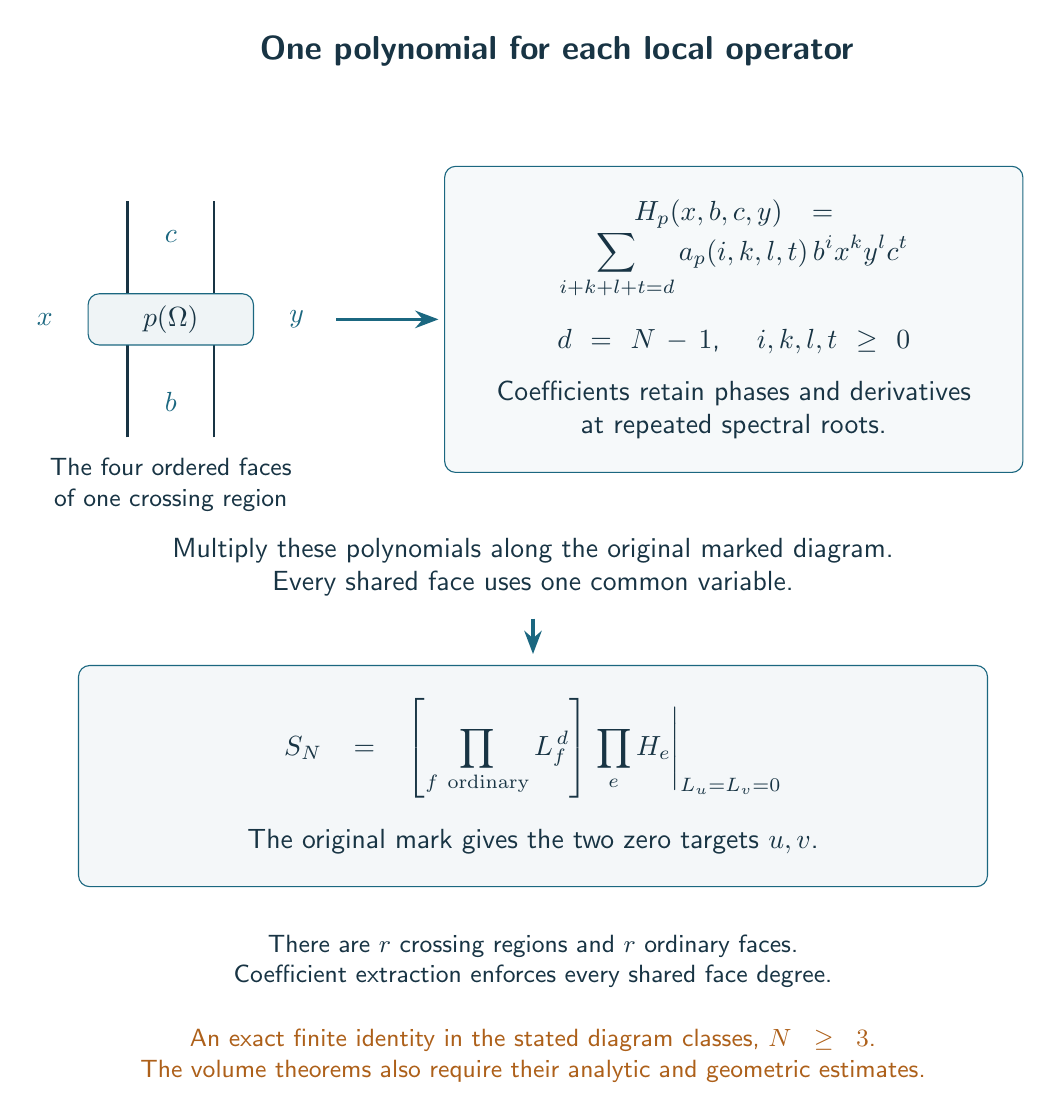
\begin{tikzpicture}[font=\sffamily,text=ink,>=Stealth]
 \node[font=\sffamily\large\bfseries] at (4.9,3.4)
 {One polynomial for each local operator};
 \draw[ink,thick] (-.55,-1.5)--(-.55,1.5);
 \draw[ink,thick] (.55,-1.5)--(.55,1.5);
 \node[draw=blue,fill=blue!7,rounded corners,minimum width=2.1cm,
       minimum height=.65cm] at (0,0) {$p(\Omega)$};
 \node[blue] at (0,1.05) {$c$};
 \node[blue] at (0,-1.05) {$b$};
 \node[blue] at (-1.6,0) {$x$};
 \node[blue] at (1.6,0) {$y$};
 \node[font=\sffamily\small,align=center] at (0,-2.1)
 {The four ordered faces\\of one crossing region};
 \draw[->,blue,very thick] (2.1,0)--(3.4,0);
 \node[draw=blue,fill=blue!4,rounded corners,align=center,
       text width=6.5cm,inner sep=12pt] at (7.15,0)
 {$\displaystyle H_p(x,b,c,y)=\sum_{i+k+l+t=d}a_p(i,k,l,t)\,
       b^i x^k y^l c^t$\\[10pt]
 $d=N-1$, \quad $i,k,l,t\geq0$\\[7pt]
 Coefficients retain phases and derivatives\\at repeated spectral roots.};
 \node[align=center,text width=10.5cm] at (4.6,-3.15)
 {Multiply these polynomials along the original marked diagram.\\
 Every shared face uses one common variable.};
 \draw[->,blue,very thick] (4.6,-3.8)--(4.6,-4.25);
 \node[draw=blue,fill=blue!5,rounded corners,align=center,
       text width=10.7cm,inner sep=12pt] at (4.6,-5.8)
 {$\displaystyle S_N=
   \left[\prod_{f\ \mathrm{ordinary}}L_f^{\,d}\right]
   \left.\prod_e H_e\right|_{L_u=L_v=0}$\\[10pt]
 The original mark gives the two zero targets $u,v$.};
 \node[align=center,text width=11.5cm,font=\sffamily\small] at (4.6,-8.15)
 {There are $r$ crossing regions and $r$ ordinary faces.\\
 Coefficient extraction enforces every shared face degree.};
 \node[amber,align=center,text width=11.5cm,font=\sffamily\small] at (4.6,-9.35)
 {An exact finite identity in the stated diagram classes, $N\geq3$.\\
 The volume theorems also require their analytic and geometric estimates.};
\end{tikzpicture}
\end{document}
